%\documentclass[options]{class}
\documentclass[10pt,journal]{IEEEtran}

%Paquete de Idioma
\usepackage[spanish, es-tabla]{babel}

%Codificación Alfabeto
\usepackage[utf8]{inputenc}

%Codificación de Fuente
\usepackage[T1]{fontenc}

%Índice
\usepackage{makeidx}

%Gráficos
\usepackage{graphicx}
\usepackage{float} 
%\usepackage{xcolor} 
\usepackage{multirow} 
\usepackage{multicol} 
\usepackage[table]{xcolor}
\usepackage[pdftex]{hyperref}
\usepackage{color}
\usepackage{colortbl}
\usepackage{authblk}
\usepackage{pgfplots}
\usepackage{mathtools}
\usepackage{graphicx}
\usepackage{subfigure}
\usepackage{hyperref}

%Matemática
\usepackage{amsmath}
\usepackage{amsfonts}
\usepackage{amssymb}
%\usepackage{amstext} 

%Estilo de Página Numeración superior
%\pagestyle{headings}

%Hiperlinks \href{url}{text}
\usepackage[pdftex]{hyperref}
\pgfplotsset{compat=1.16} 

\begin{document}
%Titulo
\title{Práctica número 1 para el uso de LaTex}
%Autor
\author
{Universidad de Guanajuato, División de Ciencias e Ingenierías\\Herramientas Informáticas y Gestión de la Información\\
Hernandez Serrano Oscar Kariel; ok.hernandezserrano@ugto.mx\\
\date{26 de abril de 2021}
}\maketitle{}
\begin{abstract}
\end{abstract} 
\section{Objetivos}
\begin{itemize}
    \item Hola
\end{itemize}
\section{Introducción}
\begin{center}
\begin{eqnarray}
\label{eq:0}
\frac{1}{2}(m+M)v_b^2=(m+M)gh
\end{eqnarray}
\end{center}\\
\begin{figure}[h]
    \centering
    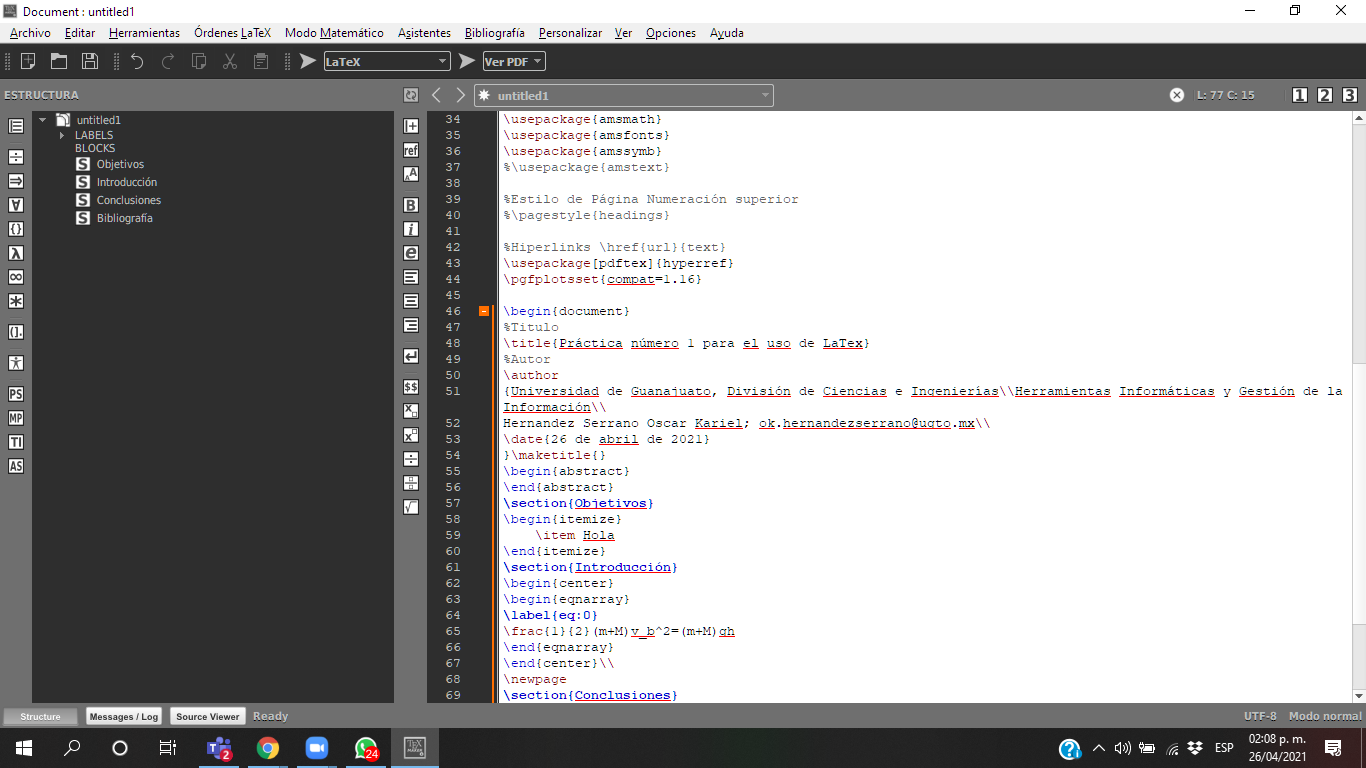
\includegraphics[width=0.4\textwidth]{Texmaker.png}
    \caption{TexMaker}
    \label{Fig. Experimento}
\end{figure}
\section{Bibliografía}
\begin{figure}[h]
    \centering
    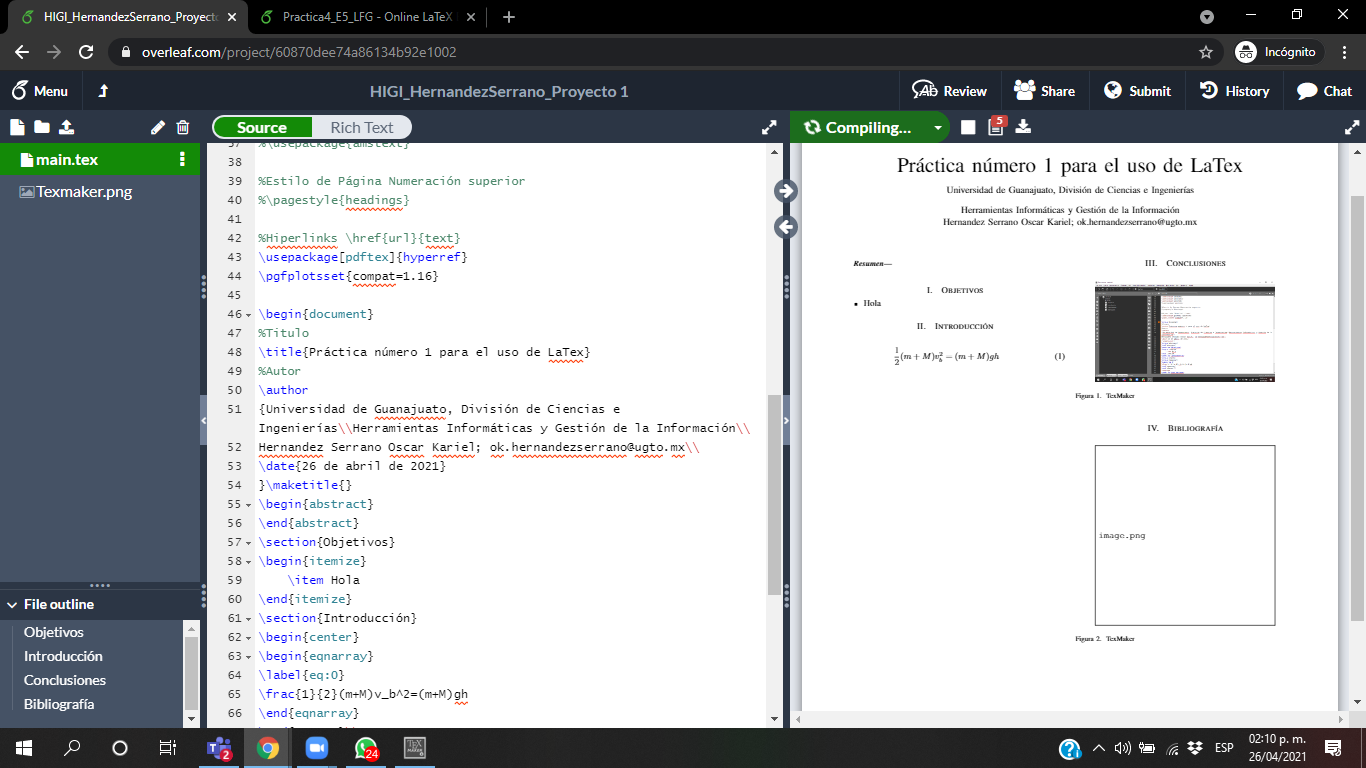
\includegraphics[width=0.4\textwidth]{image.png}
    \caption{Overleaf}
    \label{Fig. Experimento}
\end{figure}
\end{document}

